\addtocontents{toc}{\protect\setcounter{tocdepth}{0}}
\addtotoc{Management Summary}
\chapter*{Management Summary}
Exchanging data between parties is always necessary to have a functioning and robust service. This exchange process however, needs to have some sort of consistency after a while. A standardization technique for such processes must be in place.\\
\newline
The \href{https://en.wikipedia.org/wiki/European_Committee_for_Standardization}{European Committee for Standardization (CEN)} is a public standards organization that fosters the economy of the European Union (EU) in global trading and develops various technical standards for various products, materials or processes. \href{http://netex-cen.eu/}{Network Timetable Exchange (NeTEx)} is a CEN Technical Standard for exchanging public transform data. \\
\newline
In this project, we try to create a plugin for the Java OpenStreetMap editor (JOSM) that converts OpenStreetMap (OSM) data to the NeTEx format and tries to improve the OSM data by suggesting different edits for the OSM elements after the conversion has been finished. The NeTEx data is represented using XML.
\section*{Goals}
The main goal of this project is creating a JOSM plugin that grabs the currently loaded OSM map data and then does various operations in order to convert such data into the NeTEx format.\\
The plugin, during the conversion process, tries to find any inconsistencies or problems with the OSM transport data and saves them for the end of the conversion. After the conversion is completed, the plugin takes all the accumulated problems of OSM data and displays them on the JOSM map, suggesting different edits and operations for transport data that need improvement in order to stay consistent with other OSM data and with the usual approach of describing such elements.\\
This plugin also has to be published under the official JOSM plugin repository and it has to comply with the JOSM development guidelines and rules. The publishing is done for use by the community and maybe for future bug fixes or code improvements.
\section*{Results}
The plugin has been added to JOSM and has been developed and tested with real OSM data. There exists a lot of inconsistent data within JOSM, the plugin tries to fix/map such data itself during the conversion by putting different conditions, and if that data cannot be mapped or fixed by the algorithm, it means that an OSM element is missing some sort of tag that is used for identification. These elements with missing/wrong tags are displayed at the end of the conversion.\\
The plugin first takes the OSM data and creates NeTEx Java classes that have been generated by an XML binding framework, which is called JAXB and then marshalls them at the end and writes them in an XML-format file in order to complete the conversion and the export of the OSM data into NeTEx.
\begin{figure}[!htb]
	\centering
	\begin{minipage}[b]{0.48\textwidth}
		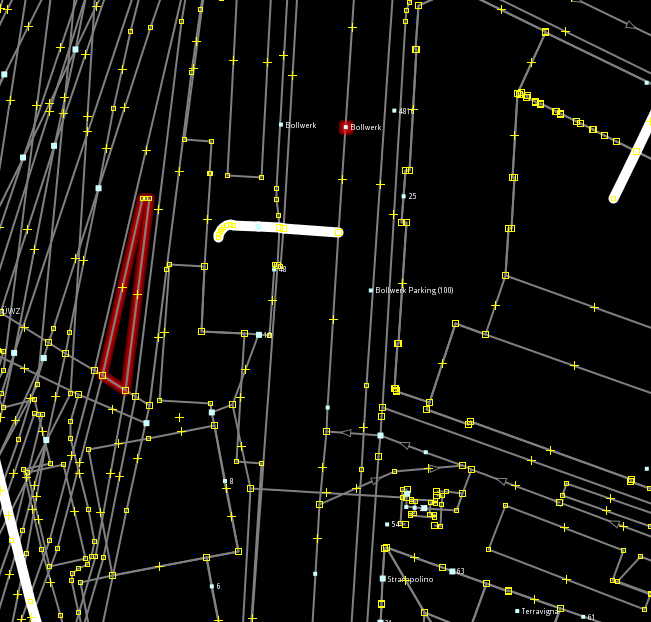
\includegraphics[width=\textwidth]{./Images/ArchitectureDesign/highlight_example.png}
		\caption{A look at how OSM elements and relations are displayed in JOSM}
	\end{minipage}
	\hfill
	\begin{minipage}[b]{0.48\textwidth}
		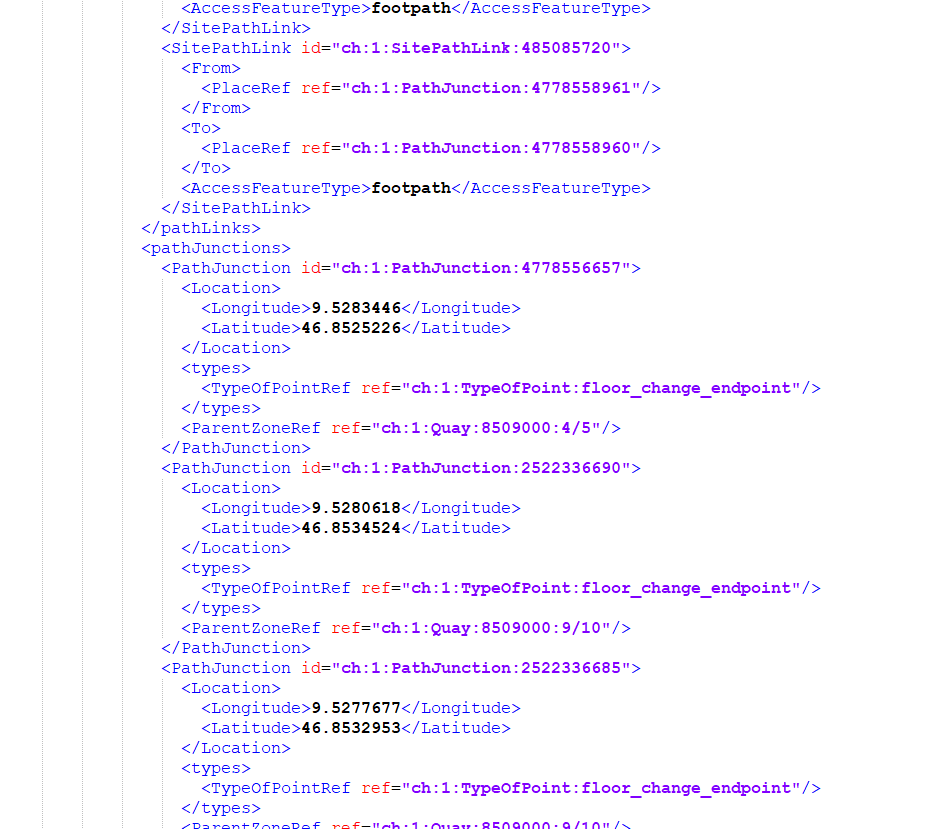
\includegraphics[width=\textwidth]{./Images/ManagementSummary/netex_doc_example.png}
		\caption{A snippet of some exported NeTEx data which was converted from OSM data using this plugin}
	\end{minipage}
\end{figure}
\newpage
\section*{Future Outlook}
The current version of this plugin successfully converts OSM data into NeTEx with a single click. Future versions can be improved in order to take care of even more conditions and data inconsistencies, improve the OSM data by providing even more suggestions etc.\\
\newline
Another very nice/important thing to add to this plugin would be implementing an algorithm for finding the associated transport objects within OSM. Some objects (like footpaths or steps) exist in or near stop places just for the purpose of leading to a platform, station etc. Such objects, don't have any tags that display what station or platform they serve. An algorithm/approach that finds such elements and their relations would be something that would improve the plugin's main algorithm by far.\\
\newline
New features can be added in the future to the plugin that would consider even more transport data (such as ferries, airports, metro stations etc) and even more NeTEx transport-related elements.